\documentclass{article}

\usepackage{fancyhdr}
\usepackage{extramarks}
\usepackage{amsmath}
\usepackage{amsthm}
\usepackage{amsfonts}
\usepackage{tikz}
\usepackage[plain]{algorithm}
\usepackage{algpseudocode}
\usepackage{graphicx}
\usepackage{listings}
\usetikzlibrary{automata,positioning}

%
% Basic Document Settings
%

\topmargin=-0.45in
\evensidemargin=0in
\oddsidemargin=0in
\textwidth=6.5in
\textheight=9.0in
\headsep=0.25in

\linespread{1.1}

\pagestyle{fancy}
\lhead{\hmwkAuthorName}
\chead{\hmwkClass\ (\hmwkClassInstructor\ \hmwkClassTime): \hmwkTitle}
\rhead{\firstxmark}
\lfoot{\lastxmark}
\cfoot{\thepage}

\renewcommand\headrulewidth{0.4pt}
\renewcommand\footrulewidth{0.4pt}

\setlength\parindent{0pt}

% \lstset{
%  columns=fixed,       
%  numbers=left,                                        % 在左侧显示行号
%  numberstyle=\small\color{gray},                       % 设定行号格式
%  frame=none,                                          % 不显示背景边框
%  backgroundcolor=\color[RGB]{245,245,244},            % 设定背景颜色
%  keywordstyle=\color[RGB]{40,40,255},                 % 设定关键字颜色
%  numberstyle=\footnotesize\color{darkgray},           
%  commentstyle=\it\color[RGB]{0,96,96},                % 设置代码注释的格式
%  stringstyle=\rmfamily\slshape\color[RGB]{128,0,0},   % 设置字符串格式
%  showstringspaces=false,                              % 不显示字符串中的空格
%  language=c++,                                        % 设置语言
% }

% \usepackage{listings}
\usepackage{color}

\definecolor{mygreen}{rgb}{0,0.6,0}
\definecolor{mygray}{rgb}{0.5,0.5,0.5}
\definecolor{mymauve}{rgb}{0.58,0,0.82}

\lstset{ 
  backgroundcolor=\color{white},   % choose the background color; you must add \usepackage{color} or \usepackage{xcolor}; should come as last argument
  basicstyle=\footnotesize,        % the size of the fonts that are used for the code
  breakatwhitespace=false,         % sets if automatic breaks should only happen at whitespace
  breaklines=true,                 % sets automatic line breaking
  captionpos=b,                    % sets the caption-position to bottom
  commentstyle=\color{mygreen},    % comment style
  deletekeywords={...},            % if you want to delete keywords from the given language
  escapeinside={\%*}{*)},          % if you want to add LaTeX within your code
  extendedchars=true,              % lets you use non-ASCII characters; for 8-bits encodings only, does not work with UTF-8
  frame=single,	                   % adds a frame around the code
  keepspaces=true,                 % keeps spaces in text, useful for keeping indentation of code (possibly needs columns=flexible)
  keywordstyle=\color{blue},       % keyword style
  language=Octave,                 % the language of the code
  morekeywords={*,...},            % if you want to add more keywords to the set
  numbers=left,                    % where to put the line-numbers; possible values are (none, left, right)
  numbersep=5pt,                   % how far the line-numbers are from the code
  numberstyle=\tiny\color{mygray}, % the style that is used for the line-numbers
  rulecolor=\color{black},         % if not set, the frame-color may be changed on line-breaks within not-black text (e.g. comments (green here))
  showspaces=false,                % show spaces everywhere adding particular underscores; it overrides 'showstringspaces'
  showstringspaces=false,          % underline spaces within strings only
  showtabs=false,                  % show tabs within strings adding particular underscores
  stepnumber=2,                    % the step between two line-numbers. If it's 1, each line will be numbered
  stringstyle=\color{mymauve},     % string literal style
  tabsize=2,	                   % sets default tabsize to 2 spaces
  title=\lstname                   % show the filename of files included with \lstinputlisting; also try caption instead of title
}

%
% Create Problem Sections
%

\newcommand{\enterProblemHeader}[1]{
    \nobreak\extramarks{}{Problem \arabic{#1} continued on next page\ldots}\nobreak{}
    \nobreak\extramarks{Problem \arabic{#1} (continued)}{Problem \arabic{#1} continued on next page\ldots}\nobreak{}
}

\newcommand{\exitProblemHeader}[1]{
    \nobreak\extramarks{Problem \arabic{#1} (continued)}{Problem \arabic{#1} continued on next page\ldots}\nobreak{}
    \stepcounter{#1}
    \nobreak\extramarks{Problem \arabic{#1}}{}\nobreak{}
}

\setcounter{secnumdepth}{0}
\newcounter{partCounter}
\newcounter{homeworkProblemCounter}
\setcounter{homeworkProblemCounter}{1}
\nobreak\extramarks{Problem \arabic{homeworkProblemCounter}}{}\nobreak{}

%
% Homework Problem Environment
%
% This environment takes an optional argument. When given, it will adjust the
% problem counter. This is useful for when the problems given for your
% assignment aren't sequential. See the last 3 problems of this template for an
% example.
%
\newenvironment{homeworkProblem}[1][-1]{
    \ifnum#1>0
        \setcounter{homeworkProblemCounter}{#1}
    \fi
    \section{Problem \arabic{homeworkProblemCounter}}
    \setcounter{partCounter}{1}
    \enterProblemHeader{homeworkProblemCounter}
}{
    \exitProblemHeader{homeworkProblemCounter}
}

%
% Homework Details
%   - Title
%   - Due date
%   - Class
%   - Section/Time
%   - Instructor
%   - Author
%

\newcommand{\hmwkTitle}{Homework\ \#1}
\newcommand{\hmwkDueDate}{Jan. 24, 2019}
\newcommand{\hmwkClass}{CPSC8400}
\newcommand{\hmwkClassTime}{}
\newcommand{\hmwkClassInstructor}{Professor Dr.Brian Dean}
\newcommand{\hmwkAuthorName}{\textbf{Guoze Tang}}

%
% Title Page
%

\title{
    \vspace{2in}
    \textmd{\textbf{\hmwkClass:\ \hmwkTitle}}\\
    \normalsize\vspace{0.1in}\small{Due\ on\ \hmwkDueDate\ at 12:25pm}\\
    \vspace{0.1in}\large{\textit{\hmwkClassInstructor\ \hmwkClassTime}}
    \vspace{3in}
}

\author{\hmwkAuthorName}
\date{}

\renewcommand{\part}[1]{\textbf{\large Part \Alph{partCounter}}\stepcounter{partCounter}\\}

%
% Various Helper Commands
%

% Useful for algorithms
\newcommand{\alg}[1]{\textsc{\bfseries \footnotesize #1}}

% For derivatives
\newcommand{\deriv}[1]{\frac{\mathrm{d}}{\mathrm{d}x} (#1)}

% For partial derivatives
\newcommand{\pderiv}[2]{\frac{\partial}{\partial #1} (#2)}

% Integral dx
\newcommand{\dx}{\mathrm{d}x}

% Alias for the Solution section header
\newcommand{\solution}{\textbf{\large Solution}}

% Probability commands: Expectation, Variance, Covariance, Bias
\newcommand{\E}{\mathrm{E}}
\newcommand{\Var}{\mathrm{Var}}
\newcommand{\Cov}{\mathrm{Cov}}
\newcommand{\Bias}{\mathrm{Bias}}

\begin{document}

\maketitle

\pagebreak

\begin{homeworkProblem}
% \textbf{Virtual Initialization}. One problem with arrays is that they must typically be initialized prior to use. On most computing environments, when we allocate an array of O(n) words of memory they start out filled with “garbage” values (whatever data last occupied that block of memory), and we must spend O(n) time setting the words in the block to some initial value. In this problem, we wish to design a data structure that behaves like an array (i.e., allowing us to retrieve the ith value and modify the ith value both in O(1) time), but which allows for initialization to a specified value v in O(1) time as well. That is, if we ask for the value of an element we have not modified since the last initialization, the result should be v. The data structure should occupy O(n) space in memory (note that this could be twice or three times as large as the actual space we need to store the elements of the array), and the data structure should function properly regardless of whatever garbage is initially present in this memory. As a hint, try to combine the best features of an array and a linked list.
    % Give an appropriate positive constant \(c\) such that \(f(n) \leq c \cdot
    % g(n)\) for all \(n > 1\).

    % \begin{enumerate}
    %     \item \(f(n) = n^2 + n + 1\), \(g(n) = 2n^3\)
    %     \item \(f(n) = n\sqrt{n} + n^2\), \(g(n) = n^2\)
    %     \item \(f(n) = n^2 - n + 1\), \(g(n) = n^2 / 2\)
    % \end{enumerate}
\textbf{Requirements}
    \begin{enumerate}
        \item Retrieve the ith valuse and modify the ith value both in O(1) time
        \item Initialization to a specified value v in O(1) time
        \item Space: O(n), can twice or three times as large as the actual space we need.
        \item The data structure should function properly regardless of whatever garbage is initially present in the memory.
    \end{enumerate}
    \textbf{Solution}

\end{homeworkProblem}

\pagebreak

\begin{homeworkProblem}
% \textbf{Enumerating Subsets by Incrementing a Binary Counter}. This is a somewhat classical amortized analysis problem. Suppose we store the digits of an n-bit binary number B in an array A of length n. We wish to increment B from 0 to $2^n - 1$ while continually modifying the contents of A to reflect the digits in B. For example, if n = 3, then we will start with $A = (0, 0, 0)$, then we toggle the last entry to obtain A = (0, 0, 1). The next increment operation changes A to A = (0, 1, 0), and so on, until we finally reach A = (1, 1, 1). Please describe how to implement the operation increment that takes an array A and modifies it by incrementing its associated binary number. Although your operation will require $\theta(n)$ time in the worst case, please show that its amortized running time is only $O(1)$ (assuming the entries in A all start out at zero). Please show how to use the accounting method as well as a potential function to perform this amortized analysis.

\textbf{Requirements}
    \begin{enumerate}
        \item Describe how to implement the operation increment
        \item Show the amortized running time in only $O(1)$ (Assum the entries in A all start out at zero)
        \item Show how to use the accounting metheod as well as a potential function to perforem this amortized analysis.
    \end{enumerate}

\textbf{Analyze}

We store the digits of an n-bit binary number B to count the incrementing and store this number to an array A of length n. And this increment counter is initially 0. The only operation is $increment(A)$. The worst case running time occurs when all k bits are flipped to 1, so $increment(A)$ has running time $O(k)$. a sequence of n increment operations, few increments will cause that many bits to flip. Suppose we do $m$ increments, we choose $m = 9$ as an example.

\begin{center}
\begin{tabular}{|c|c|c|c|c|c|c|c|c|c|c|} %l(left)居左显示 r(right)居右显示 c居中显示
\hline 
Incrementing(op\#) & 0 & 1 & 2 & 3 & 4 & 5 & 6 & 7 & 8 & ...\\
\hline 
A & (0) & (1) &(1,0) & (1,1) & (1,0,0) & (1,0,1) & (1,1,0) & (1,1,1) &(1,0,0,0) & ...\\
Flipped Number & 0 & 1 & 2 & 1 & 3 & 1 & 2 & 1 & 4 & ... \\
Cumulative & 0 & 1 & 3 & 4 & 7 & 8 & 10 & 11 & 15 & ...\\
Total(Amortized) & 2 & 2 & 2 & 2 & 2 & 2 & 2 & 2 & 2 & ... \\
New Cumulative  & 2 & 4 & 6 & 8 & 10 & 12 & 14 & 16 & 18 & ...\\

\hline 
\end{tabular}
\end{center}

In this case, the total costs is about 2m which average is 2 units per increment. Then the amortized cost per operation is O(1).

\textbf{Aggregate Method for k-increments:} K-increment for each bits:
    \begin{enumerate}
        \item bit 0 flips with every increment
        \item bit 1 flips with every $2^{nd}$ increments
        \item bit 2 flips with every $4^{th}$ increments
        \item So, the bit k flips with every $(2^k)^th$ increments
    \end{enumerate}
So the total number of bit flips in k increment operations is: 

$Total\  op = k + k/2 + k/4 ...+ k/2^k = k*(1 + 1/2 + 1/4 + ... + 1/2^k) = 2k$ 

As a result, the total cost of the sequence is O(n), then the amortized cost per operation is $O(n) / n = O(1)$$. 

\textbf{Accounting Method for k-bit:} The actual cost for an increment operation is the number of bits
flipped. We can assign an amortized cost of 2 for each increment operation. The main idea is to use 1 to flip the bit from 0 to 1 and store 1 credit to flip it back to 0 later. All changes from 1 to 0 are paid for with previously stored credit. The amortized time per operation is O(1). 

\textbf{Potential Method:} Potential Function $C_i = number$ of 1s in counter after $i^{th}$ increment. We suppose $i^{th}$ operation resets $t_i$ bits to 0.

Actual cost: $c_i = t_i + 1$

Notice That: $C_i \leq C_{i-1} - t_i + 1$. 
\begin{enumerate}
    \item If $C_i = 0, then \  C_{i-1} = t_i = k$.  
    \item If $C_i > 0, then \ C_i = C_{i-1} - t_i + 1$.  
\end{enumerate}

Difference in Potentials:

$C_i - C_{i-1} \leq (C_{i-1} - t_i + 1) - C_{i-1} = -t_i + 1$

As a result, add the actual cost, the amortized cost: $c_i + C_i - C_{i-1} \leq (t_i + 1) - t_i + 1 = 2$


\end{homeworkProblem}

\pagebreak

\begin{homeworkProblem}
% \textbf{Enumerating Permutations.} Consider a length-n array A = (1, 2, 3, . . . , n). We would like to step through all $n!$ permutations of A, updating the array as we go to represent each subsequent permutation. Permutations should be generated in lexicographic order; for example, with n = 3 we start with A = (1, 2, 3), then move to A = (1, 3, 2), A = (2, 1, 3), A = (2, 3, 1), A = (3, 1, 2), and finally A = (3, 2, 1). Please describe how to implement an operation next-perm with $O(1)$ amortized running time that modifies A to produce the next permutation in lexicographic order.Use a potential function in your analysis.
    % Write part of \alg{Quick-Sort($list, start, end$)}

\textbf{Requirements}
    \begin{enumerate}
        \item Describe how to implement an operation $next-perm$ with O(1) amortized running time that modifies A to produce the next permutation in lexicographic order.
        \item Use a potential function in the analysis.
    \end{enumerate}

\textbf{Analyze}

In order to find the next-perm base on the current number, we deal with this number from right to left. We difine the index i and j (i < j), for each index i, we want to find the first j which have $A[j] > A[i]$, swap A[i] with A[j] and reverse the A[i+1, ... n]. This operation will takes n - i + 1 times. 

\begin{lstlisting}[language=C++]
vector<int>& nextPermutation(vector<int>& A) {
  unsigned len = A.size() - 1;
  // Find an element from the right to left.
  for (int i = len - 1; i >= 0; --i) {
    if (A[i + 1] > A[i]) {
      for (int j = len; j > i; --j) {
        if (A[j] > A[i]) {
          swap(A[j], A[i]);
          reverse(A.begin() + i + 1, A.end());
          return A;
        }
      }
    }
  }
  // If there are increate order from left to right.
  reverse(A.begin(), A.end());
  return A;
}
\end{lstlisting}

As the above code, there are a few steps to find the next permutation in lexicographic order. 
\begin{enumerate}
    \item Find the largest index $i$ such that $A[i] < A[i+1]$. If no such index exists, this is the last permutation, then reverse the array A to the first permutation.
    \item Find the largest index $j$ in the $[i+1, len]$ such that $A[j] > A[i]$
    \item Swap $A[i] \  with \  A[j]$
    \item Reverse the sequence from $A[i+1]$ up to and including the final element $A[len]$
\end{enumerate}

\textbf{Potential Method:} Define the potential to be three times the length of the longest contiguously decreasing subsequence at the end of the sequence. 

\begin{enumerate}
    \item The first step costs $n-k$ (unless we have the last permutation, in which case it costs n, but that can be handled separately, since it can occur at most once in a sequence of permutations.) and does not alter the potentaial. 
    \item The seconde step costs $n-l \leq n-k$ (because k + 1 is a possible choice for l) and again does not affect the potential.
    \item  The fourth step costs n - k - 1 and replaces what was a decreasing sequence of length n - k by an ascending sequence of length n - k -but beware the fact that, with n-k = 1, the suffix has length 1 and thus can be viewed either as descending or as ascending. The potntial decreases from 3(n-k) down to 3, a decrease of 3(n-k-1). So fase, our total cost is at most 3(n-k)-1 and our decreasee in potential is 3(n-k-1), so the sum at most 2, a constant.
\end{enumerate}


The third step is the difficult one to analyze. It costs one unit of time (assuming the permutation is stored in an array), but its effect on the potential is difficult to assess. In almost all
cases, it has no effect at all. The definition of k is such that the numbers from k + 1 to n must
form a decreasing sequence; the exchange replaces the lth element, part of the decreasing suffix
sequence, with the smaller kth element, so that the new value in position l is still smaller than
the current (unchanged) (l −1)st element, but we also know that the kth element was larger than
the element at position l + 1, since that is part of the definition of l. However, in the case of
k = n− 1 and k + 1 = l = n, then the swap creates a 2-digit decreasing suffix (and the reversal
affects only the single last element and thus has no effect); that suffix could form the tail end of
a much longer (arbitrarily longer) decreasing sequence, so this step might cause an arbitrarily
large potential increase. Fortunately, each increase is matched by an equal decrease within one
step, since the potential equals 3 every other step. Thus the amortization works, but it is clearly
not any simpler than the direct analysis.

\end{homeworkProblem}

\pagebreak

\begin{homeworkProblem}
% \textbf{In-Place Matrix Transposition.} Suppose we store an $m*n$ matrix in row-major form as an array of length $N = m*n$ in which we list the elements of the matrix one row at a time from left to right. By taking the transpose of such a matrix, we convert it into column-major form - an array of length N listing the columns of the matrix one at a time, each one from top to bottom. Suppose the matrix is sufficiently large that we would like to permute its memory representation from row-major to column-major order in place (using only $O(1)$ extra storage beyond the memory that holds the matrix). Please describe and analyze an $O(N log N )$ algorithm for solving this problem. As a hint, try to design an approach modeled on the “domination radius” algorithm from lecture, noting that for each element in the matrix, you can easily determine the location to which it needs to move, as well as the location of the element that will replace it.



\textbf{Requirements}
    \begin{enumerate}
        \item Suppose the matrix is sufficiently large that we would like to permute its memory representation from row-major to column-major order in place(Space Complexity: $O(1)$).
        \item Use an $O(NlogN)$ algorithm for solving this problem.
        \item Try to design an approach modeled on the "domination radius" algorithm.
    \end{enumerate}

\textbf{Analyze}

We store an m*n matrix in row-major form as an array of length N=m*n. And transposite this matrix. There are some requirements for this question.
\begin{enumerate}
    \item Using only O(1) extra storage beyond the memory that hold the matrix.
    \item The algorithm time complexity: $O(Nlog N)$
\end{enumerate}

We use an matrix A as an example.  \\
\begin{figure}[h]
\centering
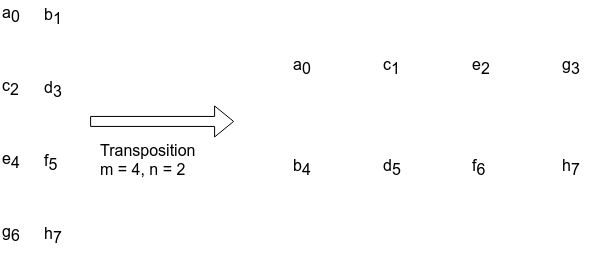
\includegraphics[scale=0.5]{images/1.png}
\end{figure}

In the above graph, small number at the right of the letter represent the index for the letter in the arrow. We can find the movement for this transposition.
\begin{lstlisting}
Index movement:
0 -> 0
1 -> 4 -> 2 -> 1
2 -> 1 -> 4 -> 2(Repetition)
3 -> 5 -> 6 -> 3
4 -> 2 -> 1 -> 4(Repetition)
5 -> 6 -> 3 -> 5(Repetition)
6 -> 3 -> 5 -> 6(Repetition)
7 -> 7
\end{lstlisting}
These index movement are 4 cycle. $0->0$,  $1 -> 4 -> 2 -> 1$, $3 -> 5 -> 6 -> 4$ and $7 -> 7$. After that, we need to think about how to find the cycle is repetition and how to calculate the precursor and successor element for the current element. \\

\textbf{Solution}

\textbf{How to know the cycle is not repetitive?}

It is easily to find whether this cycle is a repetitive cycle because we traverse this array for index 0 to N. So the first index for a new cycle which is not a repetitive one should be the lowest index in this cycle. As a result, the cycle is a repetitive cycle if there is a successor index is bigger than the first index in the cycle. 
\begin{lstlisting}[language=C++]
void transpose(int *mtx, int m, int n) {
  for (int i = 0; i < m * n; ++i) {
    int next = getNext(i, m, n);
    while (next > i)  // Detect the repetitive cycle
      next = getNext(next, m, n);
    if (next == i)  // Deal with the new cycle
      movedata(mtx, i, m, n);
  }
}
\end{lstlisting}

\textbf{How to get the precursor ans successor index?}

If the index for a element in the array is $i$ before the transposition, then the row and colume is $[i/n, i\%n]$ in the matrix. After the transposition, it change to $[i\%n,i/n]$. So the new index in the array is $(i\%n)*m + i/n$. This is the successor index for the index $i$. \\

If the index for a element in the array is $j$ after the transposition, then the row and colume is $(i/m, i\%m)$ in the matrix. Before the transposition, it is to $[i\%m,i/m]$. So the precurrsor index in the array is $(i\%m)*n + i/m$. This is the precurrsor index for the index $i$.

\begin{lstlisting}[language=C++]
int getNext(int i, int m, int n) { return (i % n) * m + i / n; }
int getPre(int i, int m, int n) { return (i % m) * n + i / m; }
\end{lstlisting}

\textbf{How to move the elements in a new cycle?}

\begin{lstlisting}[language=C++]
void movedata(int *mtx, int i, int m, int n) {
  int temp = mtx[i];
  int cur = i;
  int pre = getPre(cur, m, n);
  while (pre != i) {
    mtx[cur] = mtx[pre];
    cur = pre;
    pre = getPre(cur, m, n);
  }
  mtx[cur] = temp;
}
\end{lstlisting}

This algorithm has time complexity: $O(n^2)$ and space complexity: $O(1)$. We can think about use the domination radius method to detect the cycle both left and right at the same time. Then we can reduce the time complexity to $O(n log n)$.

\begin{lstlisting}[language=C++]
void transpose(int *mtx, int m, int n) {
  for (int i = 0; i < m * n; ++i) {
    int pre = getPre(cur, m, n),  next = getNext(i, m, n);
    while(pre > i && next > i && pre!= next && getPre(m, n, pre) != next) {
      pre = getPre(m,n,pre);
      next = getNext(m,n,next); 
    }
    if(pre < i || next < i) continue;
    movedata(mtx, i, m, n);
  }
}
\end{lstlisting}

\end{homeworkProblem}


\end{document}
